\section{Introduction}

Single-particle cryo-electron microscopy (cryo-EM) has revolutionized the field of structural biology over the last decades~\cite{dubochet1988cryo, frank2006three,chap0-nat2015MethodYear}. The use of electron beams to image ice-embedded samples has permitted the recovery of 3D bio-structures at unprecedented resolution. This advent of atomic-resolution cryo-EM has had a tremendous impact in biomedical research, providing invaluable insights into the biological processes that underlie many current diseases.

In single-particle cryo-EM, every 3D particle adopt a random orientation in the ice layer before being imaged with parallel beams of electrons.
Hence, the projection geometry associated to each acquired 2D projection (\figref{imaging-geometry}) is unknown. Yet, this knowledge is essential for the tomographic reconstruction of bio-structures~\cite{Natterer2001mathematics}.

\tdplotsetmaincoords{60}{110}
\pgfmathsetmacro{\rvec}{.8}
\pgfmathsetmacro{\thetavec}{30}
\pgfmathsetmacro{\phivec}{60}
\begin{figure}
\centering
\begin{tikzpicture}[scale=4,tdplot_main_coords]
    \coordinate (O) at (0,0,0);
    \draw[thick,->] (0,0,0) -- (1,0,0) node[anchor=north east]{$\bsx_1$};
    \draw[thick,->] (0,0,0) -- (0,1,0) node[anchor=north west]{$\bsx_2$};
    \draw[thick,->] (0,0,0) -- (0,0,1) node[anchor=south]{$\bsx_3$};
    \tdplotsetcoord{P}{\rvec}{\thetavec}{\phivec}
    \draw[-stealth,very thick,color=red] (O) -- (P);
    \draw[dashed, color=red] (O) -- (Pxy);
    \draw[dashed, color=red] (P) -- (Pxy);
    \tdplotdrawarc{(O)}{0.2}{0}{\phivec}{anchor=north}{$\theta_1$}
    \tdplotsetthetaplanecoords{\phivec}
    \tdplotdrawarc[tdplot_rotated_coords]{(0,0,0)}{0.5}{0}%
        {\thetavec}{anchor=south west}{$\theta_2$}
    \draw[dashed,tdplot_rotated_coords] (\rvec,0,0) arc (0:90:\rvec);
    \draw[dashed] (\rvec,0,0) arc (0:90:\rvec);
    \tdplotsetrotatedcoords{\phivec}{\thetavec}{0}
    \tdplotsetrotatedcoordsorigin{(P)}
    \draw[dashed,blue,tdplot_rotated_coords,-] (-.4,0,0)
        -- (.4,0,0) node[anchor=north west]{};
    \draw[dashed,blue,tdplot_rotated_coords,-] (0,-.4,0)
        -- (0,.4,0) node[anchor=west]{};
    \draw[blue,tdplot_rotated_coords,-]  (-.4,.4,0) -- (.4,.4,0)  -- (.4,-.4,0) -- (-.4,-.4,0) -- (-.4,.4,0)   node[anchor=north]{};
    \tdplotdrawarc[tdplot_rotated_coords]{(0,0,0)}{0.2}{0}%
        {30}{anchor=north west,color=black}{$\theta_3$}
    \tdplotsetrotatedcoords{\phivec}{\thetavec}{30}
    \draw[thick,tdplot_rotated_coords,->] (0,0,0)
        -- (.3,0,0) node[anchor=north west]{$\bsy_1$};
    \draw[thick,tdplot_rotated_coords,->] (0,0,0)
        -- (0,.3,0) node[anchor=west]{$\bsy_2$};
    \node[blue] at (0.4,0.45,1.2) {$\Omega_{\mathrm{2D}}$};
    \node[red] at (1.5,0.75,1.2) {$\bvth_{\bth}$};
    \tdplotsetrotatedthetaplanecoords{45}
\end{tikzpicture}
\caption*{\mdeff{Kept as reference for \figref{imaging-geometry} as this tikz figure is beautiful. Will be commented out in the end.}}
\end{figure}

\begin{figure}
    \centering
    \begin{subfigure}[t]{0.45\linewidth}
        \centering
        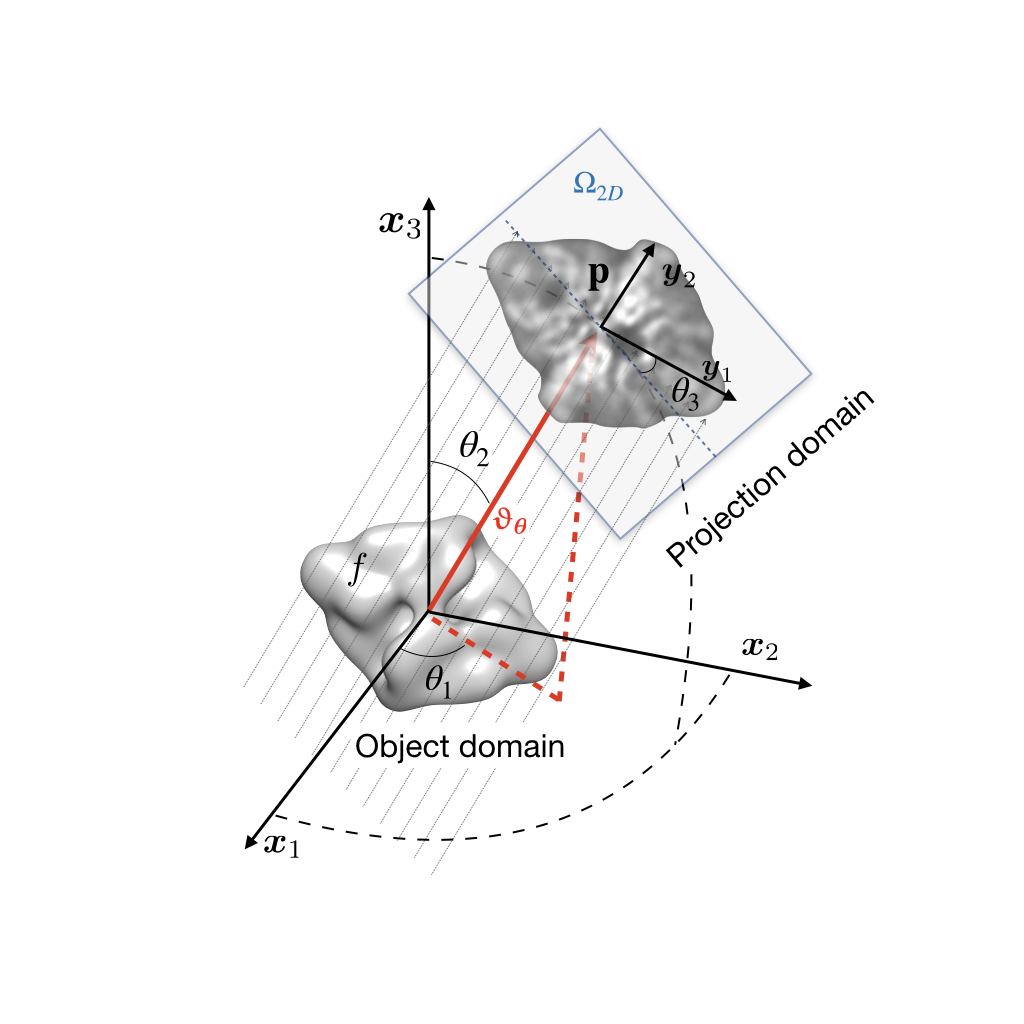
\includegraphics[height=7cm]{geomProj3D001}
        \caption{
            \banjac{pdf is losing the colors, therefore png export type.} \mdeff{That's unfortunate because this figure is beautiful. Laurène, any idea why?}
            \todo{Coordinates $(x_1, x_2, x_3)$ and $(y_1, y_2)$ in non-bold face.}
            \todo{$y_1, y_2, \theta_3, \theta_1$ would be more visible out of the darker part.}
            \todo{Object (or protein?) $\mathbf{x}$ (not $f$) and projection $\mathbf{p}$. Keep or remove ``domain''?}
            \todo{Remove $\Omega_{2D}$?} % $\Omega_{\mathrm{2D}}$ with 2D not italic.}
            \todo{Extend $x_1$ and $x_2$ for elevation ($\theta_2$ dashed gray line) to not look ``squashed''.}
            \todo{The vertical red line should be parallel to the $x_3$-axis.}
            \todo{Remove $\bvth_{\bth}$.}
        }\label{fig:imaging-geometry}
    \end{subfigure}
    \qquad
    \begin{subfigure}[t]{0.45\linewidth}
        \centering
        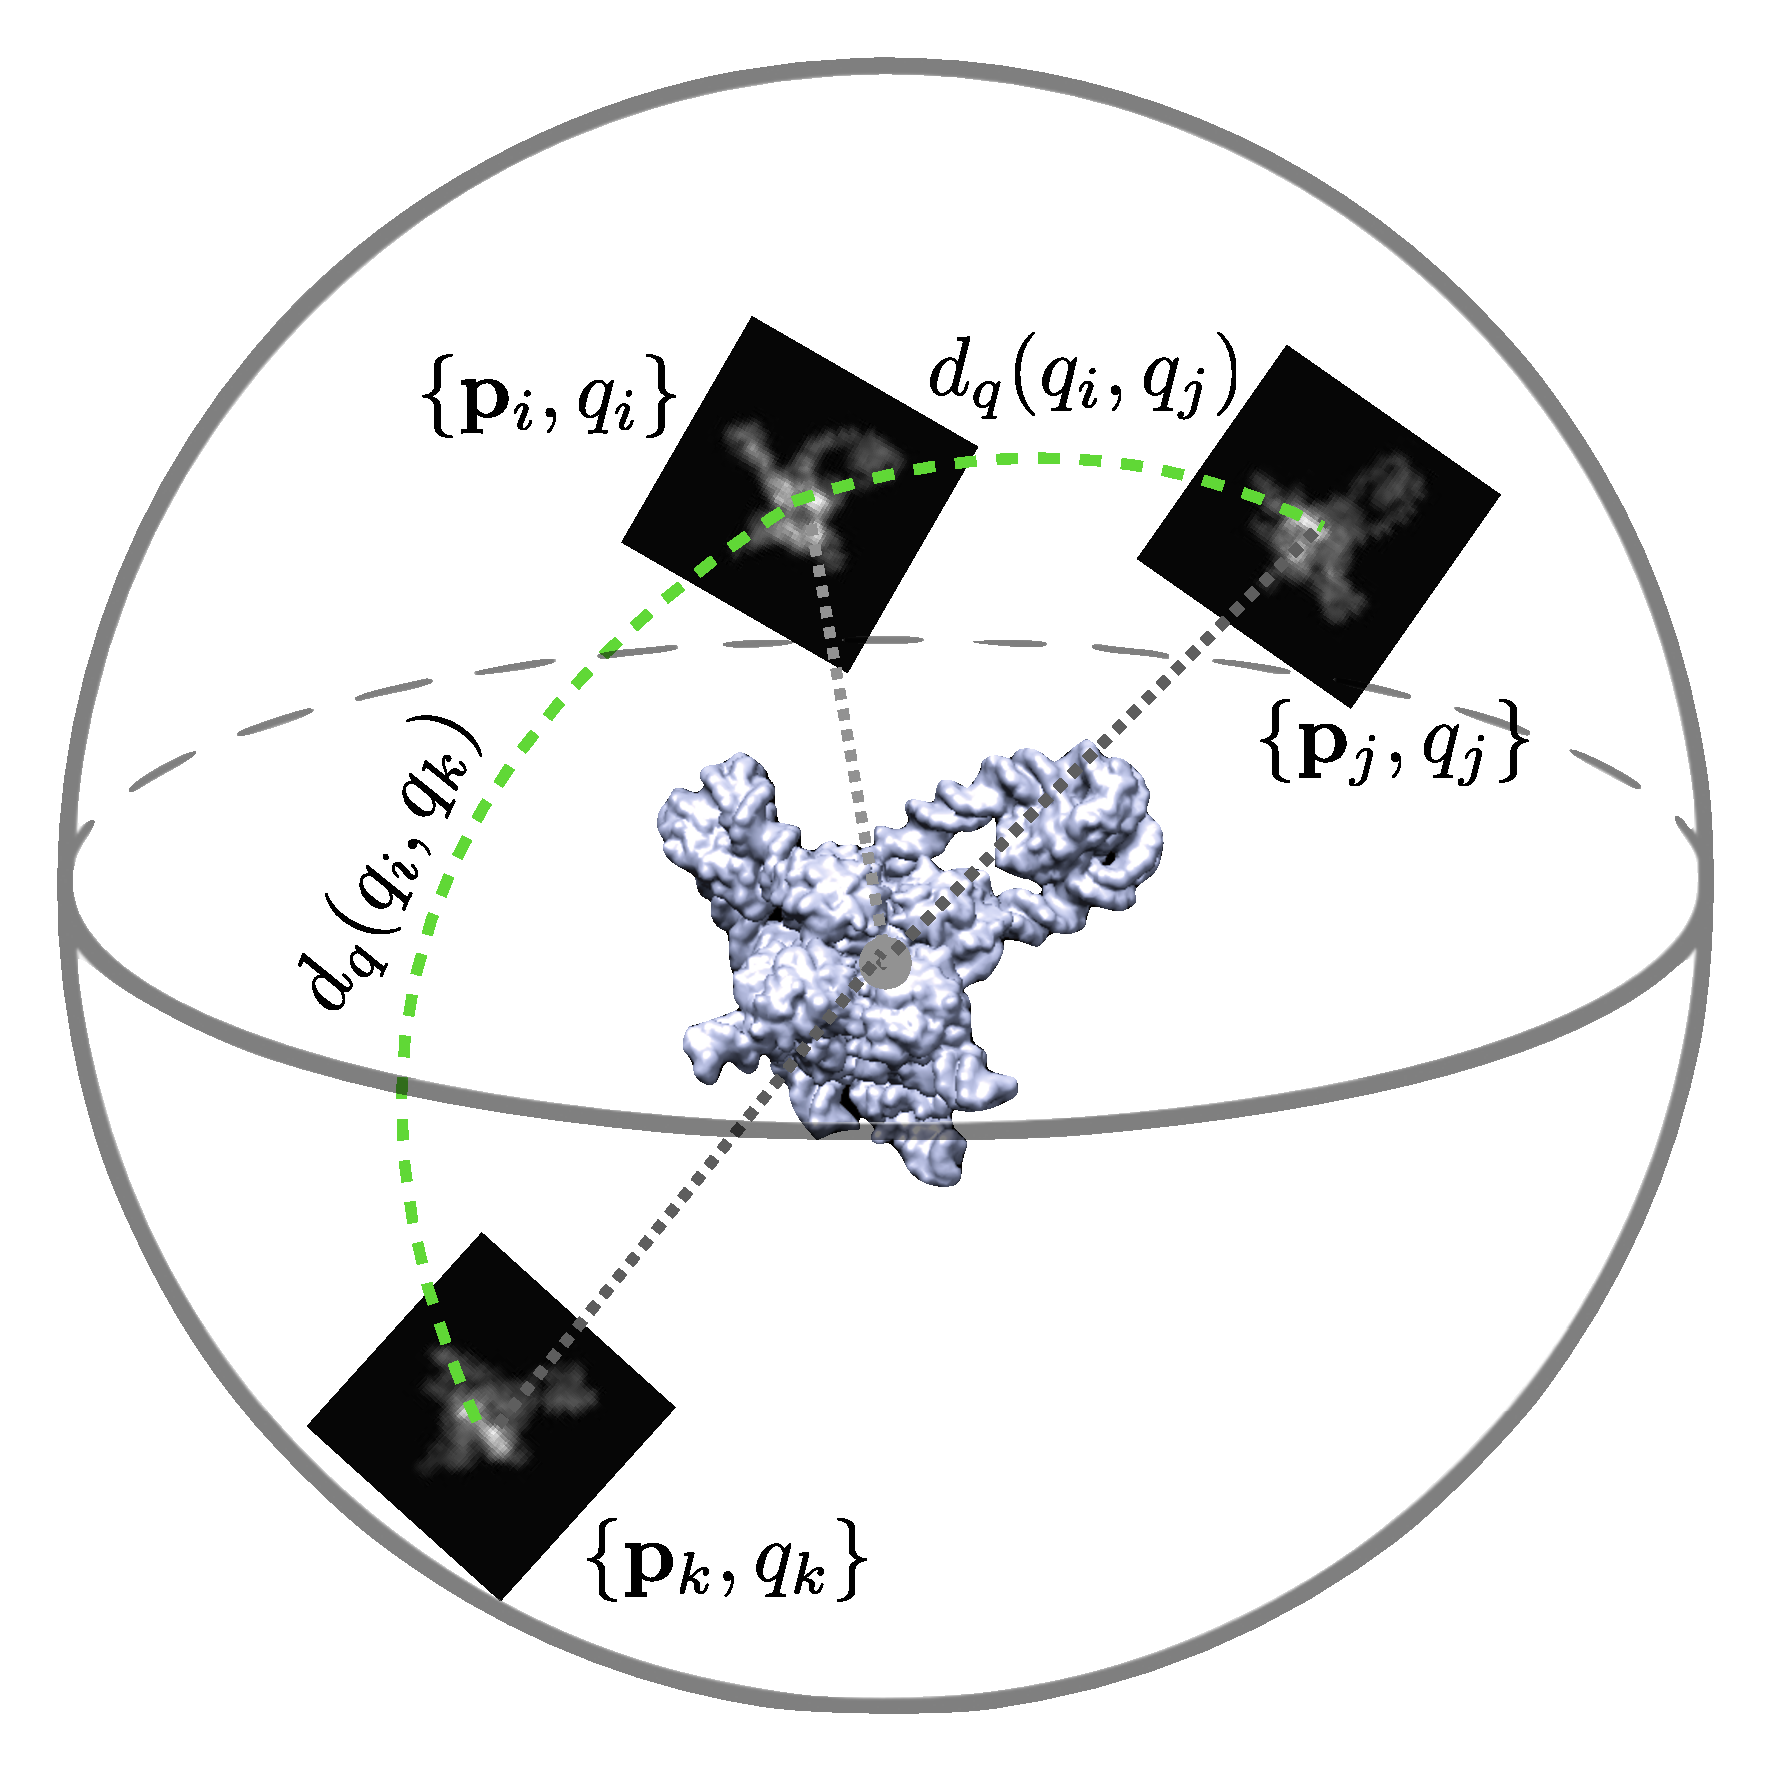
\includegraphics[height=7cm]{intuition_method}
        \caption{
            \todo{$(\p_i, qi)$ with parentheses instead of braces (ordered tuples, not sets).}
            \todo{Consistent color for $d_q$ (text and arc) with \figref{schematic:method-overview}.}
            \todo{The projections don't look to be on the surface of the sphere: They should be on tangent planes.}
            \todo{The gray line to the center is the projection direction to be labeled $(\theta_1, \theta_2)$ with a color consistent with \figref{imaging-geometry}.}
            \todo{The two green arcs seems too much like a single one.}
            \todo{Show also $d_q(q_j, q_k)$ (there's otherwise not enough constraints and an infinite number of solutions).}
            \todo{The sphere lines should be finer.}
        }\label{fig:intuition-method}
    \end{subfigure}
\caption{%
    % Goals: explain
    % * (i) what we mean by a projection and an orientation (the two most important objects of our paper), and
    % * (ii) how a projection (=integration through z in the new coordinate system) is made from a 3D volume.
    \textbf{Projections and orientations.}
    (a) Geometry of the imaging model $\p = \mathbf{P} \Rot(\bth) \x$ \todo{($\mathbf{P}$ is a projection/integration)}.
    The 3D object \mdeff{(protein or particle for consistency?)} $\x$ in the coordinate system $(x_1, x_2, x_3)$ is imaged along the direction $\bvth_{\bth}$ \mdeff{Ok with ``direction $(\theta_1, \theta_2)$''? (I'd prefer to not introduce notation we won't use.)} to produce the 2D \textit{projection} $\p$ in the coordinate system $(y_1, y_2)$.
    The direction $(\theta_1, \theta_2) \in [0,2\pi[ \, \times \, [0,\pi]$ (parameterizing the sphere $\mathbb{S}^2$) and the in-plane rotation $\theta_3 \in [0,2\pi[$ (parameterizing the circle $\mathbb{S}^1$) forms the \textit{orientation} $\bth = (\theta_1, \theta_2, \theta_3)$.
    Alternatively, we represent the orientation $\bth$ as a unit quaternion $q$.
    %$\bth = (\theta_1, \theta_2, \theta_3)$ are the rotation $\theta_1$, the tilt \todo{or azimuth?} $\theta_2$, and the in-plane rotation $\theta_3$.
    The 3D rotation $\Rot(\bth) = \Rot(q) \in \SO(3)$ maps the object coordinate system to the projection coordinate system.
    \mdeff{$\Rot$, $\bth$, and $q$ all represent orientations. That's the problem with notation that separates the representation not the semantic (though we might need that separation later).}
%    The set $\Omega_{\mathrm{2D}}$ denotes the support of the projection.
%    \mdeff{Is $\Omega_{\mathrm{2D}}$ a set? Not a vector space?} \lau{It is a set in the way I define it in my thesis, but we can remove the word if you find it confusing here.}
    (b) Single-particle cryo-EM produces $P \approx 10^5$ projections, taken from unknown orientations: $\{(\p_i, q_i)\}_{i=1}^P$.
    Observing that distances between points constrain their position, we aim to \textit{recover the orientations} $\{q_i\}$ from the distances $\{d_q(q_i, q_j)\}$.
    Observing that projections taken from close orientations look alike, we aim to \textit{estimate the distances} $\{d_q(q_i, q_j)\}$ from the projections $\{(\p_i, \p_j)\}$.
    \mdeff{Easy to see that the geodesic distance $d_q$ is the amplitude of a rotation between two orientations.}
}
\end{figure}

% RELATED WORKS
To handle this, a popular approach in single-particle cryo-EM is to alternatively refine the 3D structure and the estimation of the orientations~\cite{penczek1994ribosome,Baker1996,Dempster1977,sigworth1998maximum,scheres2012bayesian,zehni2020joint}. Unfortunately, the outcome of these iterative-refinement procedures is most often predicated on the quality of the initial \textit{ab initio} reconstruction, or, equivalently, on the initial estimation of the orientations~\cite{sorzano2006optimization,henderson2012outcome}.

Several methods have been designed to produce a first rough \textit{ab initio} structure for the refinement procedure~\cite{singer2020computational}. An early approach~\cite{kam1980reconstruction} proposed to reconstruct an initial structure such that the first few moments of the distribution of its theoretical measurements match the ones of its experimental projections. Since then, \textit{moment-matching} techniques have been refined and extended~\cite{salzman1990method,goncharov1988integral,sharon2019method}, \textit{e.g.}, to accommodate for non-uniform orientation configurations. However, they typically remain sensitive to error in data and can require relatively high computational complexity.  %If needs be for downside: relatively important computational complexity, and remain sensitive to error in data.

Another popular line of approach in single-particle cryo-EM  relies on the central-slice theorem, which relates the Fourier transform of a projection to a plane (orthogonal to the projection direction) in the Fourier transform of the 3D object~\cite{Natterer2001mathematics}. Hence, every two projections \textit{de facto} share a common 1D intersection in the 3D Fourier domain, and three projections theoretically suffice to define a coordinate system from which their orientations can be deduced~\cite{van1987angular}. Exploiting this principle, \textit{common-lines} methods aim at uniquely determining the orientations of each projections by identifying the common-lines between triplets of projections~\cite{penczek1994ribosome,mallick2006structure,singer2010detecting,wang2013orientation,greenberg2017common,pragier2019common}---a real technical challenge given the massive amount of noise in cryo-EM data. %If needs be for downside: sensitivity to high-noise levels, small particles, etc.

Alternatively, the  marginalized maximum likelihood (ML) formulation of the reconstruction problem---classically used for the iterative-refinement procedures themselves---can be minimized using stochastic gradient descents~\cite{punjani2017cryosparc}. This permits to avoid the need for an initial volume estimate, at the possible cost of greater convergence instability. More recently, the recovery of geometrical information from unknown view tomography of 2D point sources has been proposed~\cite{zehni2019distance}, but the extension to 3D cryo-EM tomography is not straightforward yet.

Hence, despite the many aforementioned advances, the task of providing a robust initial volume remains a notoriously arduous challenge in single-particle cryo-EM due to the high-dimensionality and strong ill-posedness of the underlying optimization problem.

%\mdeff{Content. (p1) Why is the general problem of protein reconstruction important and difficult. (p2) Short background on single-particle cryo-EM and how reconstruction is done. (p3) Previous work on orientation estimation (or initial structure estimation). If there's none (because people have researched other routes), state it and write why it's an interesting route to explore. How does it compare to initial rough structure estimation? Or whatever the other routes are. (p4) Our contribution on top of previous work.}
